\documentclass[a4paper,twoside]{article}

\usepackage{epsfig}
\usepackage{pdfpages}
% \usepackage{subfigure}
\usepackage{calc}
\usepackage{amssymb}
\usepackage{amstext}
\usepackage{amsmath}
\usepackage{amsthm}
\usepackage{bm}
% \usepackage{enumitem}
% \usepackage{commath}
\usepackage{multicol}
\usepackage{xcolor}
\usepackage{graphicx}
\usepackage{pslatex}
\usepackage{apalike}
\usepackage{SCITEPRESS}
\usepackage[small]{caption}
\usepackage{hyperref}


\graphicspath{{./figures/}}



\newcommand{\SC}[1]{{\color{blue}SC: #1}}

\title{Detection, Tracking, and Prediction of Events Using Micro-Blogs}

\author{
    \authorname{Shobhit Chaurasia\sup{1}, Harshil Lodhi\sup{1}, Nishant Yadav\sup{1} and Sanasam Ranbir Singh\sup{1}}
    \affiliation{\sup{1}Indian Institute of Technology Guwahati}
    \email{\{c.shobhit,harshil,nishant.yadav,ranbir\}@iitg.ernet.in}
}

\begin{document}
\includepdf{cover.pdf}
\includepdf{certi.pdf}
\keywords{Topic Models, Latent Dirichlet Allocation, LDA, Twitter, Event Detection, Event Evolution, Event Prediction}

\abstract{
We describe our semester long work on Event Detection and Tracking on Twitter. We have presented a survery of the available literature in this field. We have evaluated various different modelling techniques for twitter data and have reported results for each of them. We discuss the future work which we plan to do to achieve our objective.
%
}


\onecolumn \maketitle \normalsize \vfill

\section{\uppercase{Introduction}}
Humans have a curiosity to know more about their surrounding environment. This need for information is the main factor that has contributed towards the survival of human race. For instance, the news of the outbreak of an epidemic is immediately followed by the adoption of additional health care measures by people living in the affected regions. This huge appetite for information was originally satisfied by written media like newspapers, telegraphs etc. Then, with advancements in technology came television and telephones which provided information at a much faster rate. In the present generation, the growth of Internet has completely changed the way information is shared and received. This increase in popularity and need for information sharing has led to the emergence of social networking platforms like Twitter.

Twitter has a huge user base sharing all kinds of information at a very high rate. Information shared on Twitter range from personal information like what they are eating, to local events like festival celebrations, to events having worldwide impact like forest fires. Since the users of Twitter are spread all over the world, and people usually Tweet about events almost instantaneously, it can be considered as a large media company having its reporters spread all over the world reporting events 24*7. This fact makes the study of Twitter data very important in order to model the evolution of important events through tweets. However, along with the diversity and richness of information pervading the Twitter ecosystem comes an equally huge amount of uninteresting, insignificant and noisy information, such as updates about daily chores of a user. Mining useful information from this exploding space of tweets calls for meticulous organization and structuring of data. With this motivation, we wish to explore the problem of detection, tracking, and prediction of events using micro-blog posts.

The rest of the report is organized as follows. We begin by presenting our problem statement in a formal manner in Section 2. This is followed by a discussion on the Twitter ecosystem in Section 3. Section 4 presents a brief overview of Latent Dirichlet Allocation. In Section 5, we present a comprehensive review of the numerous techniques which have been proposed in literature for the purpose of event detection in Twitter. 

This is followed by a brief discussion of Twitter LDA in Section 6, which is an interesting variant of LDA build for inferring topic distributions on Twitter data.
\section{\uppercase{Problem Definition}}
No idea :P
\section{\uppercase{Understanding Twitter Ecosystem}}
In this world of big data, no one can ignore the impact that Twitter has in terms of data availablibity and data processing. On a typical day, more than 500 million tweets are posted. This amount of data was never available before. The traditional media like newspaper, articles, magazines are very different from Twitter data. Tweets provide almost real-time information and discussions of current events. However, tweets are highly fragmented and noisy, and contain non-interesting events as well, such as personal musings of users about their day-to-day activities. Moreover, the informal, ill-framed, and unstructured nature of messages adds to the noise. All these characteristics of tweets make it difficult for the traditional systems which were based on carefully written and well-structured news articles to process Twitter data. Tweets mostly contain different spellings and misspellings for a single word. Because of the 140 character limit, most of the users refrain from the use of proper punctuations and stop-words in their tweets, resulting in grammatically, semantically and syntactically messy texts.

If we consider tweets about users' daily mundane tasks, these tweets come up on Twitter in a large volume on any given day. Intermixed with this uninteresting volume of tweets is a set of equally bursty and information-rich tweets about important events. So, to differentiate between these two classes of tweets, one cannot directly use the frequency; temporal/spatial features of these class of tweets need to be considered. Tweets consisting of daily mundane tasks are evenly distributed across the timeline while tweets about important events are concentrated to a certain part of the temporal and/or spatial dimension.

\paragraph{Events}
To define an \emph{event}, we need to state what a topic is. Quoting from \cite{zhao2011comparing}, \textquotedblleft A topic is a subject discussed in one or more documents\textquotedblright. An \emph{event} is an abstract idea which has a topic, a temporal dimension, a spatial dimension, and/or entities associated with it. For example, \textquotedblleft Death of Steve Jobs\textquotedblright~was trending at Twitter. This event has a topic \textquotedblleft death\textquotedblright~which is associated with an entity \textquotedblleft Steve Jobs\textquotedblright~and it has a temporal dimension since the burst of tweets appeared in the first week of October, the time when Steve jobs died. The temporal and spatial dimensions can be found explicitly from the tweet content and/or from the tweet's meta-data. A topic alone cannot define an event. So, to make sense from the data, one first needs to find out the different topics from the given data and then, figure out whether there is an associated entity, or a temporal/spatial dimension to it or not.
 \begin{figure*}
 \centering
 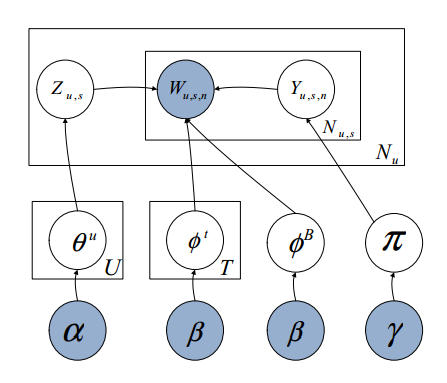
\includegraphics[width=0.5\textwidth]{figures/twitter-lda}
 \caption{Twitter LDA Plate Notation}
 \label{fig:plate}
\end{figure*}

\section{\uppercase{Latent Dirichlet Allocation}}
Latent Dirichlet Allocation (LDA) is a probabilistic generative model which automatically and jointly clusters words into topics and documents into mixture of topics.

LDA assumes that documents are a mixture of topics which give out words with certain probabilities. The generative process is defined below:
\begin{enumerate}
\item Decide on the total number of words that a document will have, lets say $N$ and there are $M$ no. of documents.
\item Choose $\theta_i \, \sim \, \mathrm{Dir}(\alpha)$ , where $i$ $\in$ $\{ 1,\dots,M \}$ and $\mathrm{Dir}(\alpha)$  is the Dirichlet distribution for parameter $\alpha$.
\item Choose $\phi_k \, \sim \, \mathrm{Dir}(\beta)$ , where  $k \in \{ 1,\dots,K \}$ .
\item For each of the word positions $i, j,$ where  $j \in \{ 1,\dots,N_i \}$ , and  $i \in \{ 1,\dots,M \} $.
\begin{itemize}
\item Choose a topic $z_{i,j} \,\sim\, \mathrm{Multinomial}(\theta_i)$. 
\item Choose a word $w_{i,j} \,\sim\, \mathrm{Multinomial}( \phi_{z_{i,j}})$.
\end{itemize}
\end{enumerate}


\section{\uppercase{Literature Review}}
\subsection{\uppercase{Event Detection}}
{\bf Shobhit Chaurasia} and {\bf Harshil Lodhi} have equally contributed to exploring state-of-the-art techniques proposed in literature for the purpose of event detection using Twitter data. They have comprehensively explored techniques to improve the performance of topic models, in particular LDA, on Twitter data.

In recent years, a lot of work has been done in mining hot/trending topics from Twitter stream. Twitter itself shows Trending Topics in its feed. \cite{lee2011twitter} have proposed extensions to this framework by classifying Trending Topics on Twitter using text-based and network-based classifiers. Recently, the focus in literature has shifted beyond the identification of trending topics; the problem of real-world event detection using social media has started receiving overwhelming attention. Researchers have explored the domain of event identification using social media updates, specifically Twitter. While some efforts have focused upon event detection in general \cite{becker2010learning}, other efforts have been directed towards detection of particular class of events such as earthquakes \cite{sakaki2010earthquake}, news reports \cite{sankaranarayanan2009twitterstand}. To this end, numerous techniques have been exploited. While \cite{becker2010learning} have explored ensemble-based clustering methods for learning similarity metrics for clustering related tweets, \cite{becker2011beyond} have focused on online identification of events using classification techniques. One special technique which has gained our attention, and which we have been exploring is using Topic Models on Twitter data for detection of events.

Topic modeling of the news-wire data has seen a lot of success. Topic modeling techniques such as LDA performs very well on the news data where a document is actually a mixture of a large number of topics. However, the standard LDA doesn't work well on the Twitter data, the major problem being that if we consider a tweet as a single document, then the document is too sparse for the LDA. The most commonly exploited technique to improve the performance of LDA on Twitter data is the aggregation of tweets which are similar in some sense or the other, such as temporally, linguistically, spatially and semantically, so as to feed the topic model with more content-rich documents enabling better topic inferences.

Several attempts have been made to extend LDA to better capture topics in micro-blogs and tweets. \cite{hong2010empirical} have analyzed different tweet aggregation techniques for training the topic models, in particular, LDA and the Author-Topic (AT) model \cite{rosen2004author}. The AT model extends LDA by modeling each word in the document as being latently associated to a topic $z$ as well as an author $x$. An author $x$ is a multinomial ($\theta$) over topics, which in turn is a multinomial distribution ($\phi$) over the words $w$ of the vocabulary. Unlike LDA, where only the words are observed, in AT model, both words and authors are observed. Three schemes have been discussed for training the topic models.
\begin{enumerate}
\item {\bf MSG scheme:} The focus here is the tweet itself. LDA is trained on all the tweets. For training purposes, each tweet is considered individually as a document.
\item {\bf USER scheme:} The focus here is the user. The model is not trained on individual tweets; rather, aggregation of all tweets of a particular user is fed to the model as a document.
\item {\bf TERM scheme:} This is a rather non-intuitive scheme, where tweets are aggregated based on the terms they contain. For each term, all the tweets containing that term are aggregated. Each document thus contains tweets that have a particular term in common.
\end{enumerate}

The inherent differences in the properties of each scheme can potentially lead to different topic proportions being inferred for the same testing set. For example, under \emph{MSG scheme}, model in trained on individual tweets, which are very short. Hence, more numbers of topics are needed for a reasonable performance. Training set for \emph{USER} and \emph{TERM schemes} have sufficiently large documents. The intuition behind the \emph{TERM scheme} is to capture the topics represented directly by the hashtags in tweets. Further, the authors use JS divergence to measure the similarity between the topics inferred by the three different schemes.

\cite{mehrotra2013improving} have examined additional tweet pooling schemes, including Burst-score wise pooling, Temporal pooling, and hashtag-based pooling. In Burst-score wise pooling, for each burst term, tweets possessing that term are pooled together into one document. Temporal pooling tries to capture the simultaneous tweets posted by users in wake of an occurrence of a major event by concatenating tweets posted within the same hour to form a document. The resulting topic inferences were found to be best in case of hashtag-based pooling. This result is quite intuitive, since hashtags inherently represent the context of the tweets; they are topics in disguise, and can be viewed as indirect topic assignment by the humans themselves. However, as noted, only a small portions of tweets are hash-tagged. Moreover, hash tags may not cover all the topics related to the tweet.

LDA as a model is unsupervised in nature. It does not need any labeled documents for the purpose of topic inferences. \cite{ramage2009labeled} have proposed Labeled LDA, a supervised version of the standard LDA, wherein a set of labels are provided as parameter to the model to be used as observed parameters for assigning topics to the documents. \cite{ramage2010characterizing} have explored the nature of Twitter messages and classified them into five different categories. Among these categories, the category of interest to us is the \emph{substance category}, which encompasses tweets about events, ideas, things, or people. They have used Labeled LDA to explore latent dimensions in Twitter posts, and further project these dimensions to the five categories. Further, to exploit the supervised learning aspect of Labeled LDA, they have used labels derived from hashtags, emoticons and Twitter meta-data like replies and temporal information to train the model. The combination of the latent features, and labeled features, and their projection to the \emph{substance category} could potentially lead to very accurate topic-to-event mapping which we are aiming to achieve.

 \begin{figure*}
 \centering
 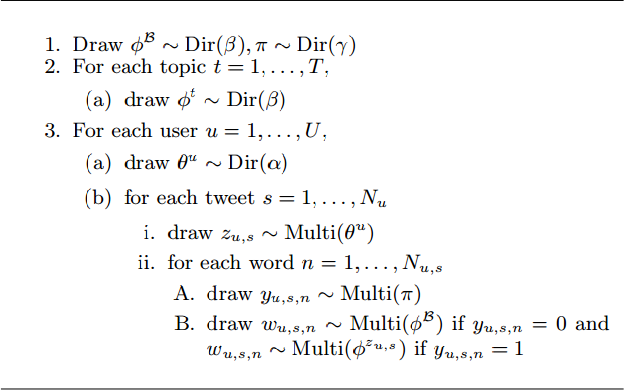
\includegraphics[width=0.6\textwidth]{figures/lda-algo}
 \caption{Twitter LDA Generative Process}
 \label{fig:twitterlda-algo}
\end{figure*}

Numerous research efforts have proposed approaches which are branches of the topic modeling paradigm, enhanced by use of other novel techniques and orthogonal ideas. \cite{wang2013real} have employed Gaussian mixture for choosing bursty words as potential candidates for being associated to an event. To further evaluate their candidacy, they have employed evolutionary clustering to model the temporal evolution of the candidate topics, before declaring them as being tightly-coupled to an event. They have proposed a time dependent HDP, which is an extension of a yet another powerful topic model - Hierarchical Dirichlet Process (HDP). Similarly, \cite{you2013geam} have come up with an Aspect Model called GEAM (General and Event-related Aspect Model) for extracting events information from noisy Twitter data.

With so many model proposals in the literature for event detection based on Twitter data, our focus is to tune the proposed models to fit our requirements - detection of non-popular events. While many methods are agnostic to popularity or bursty nature of the events being detected, others directly or indirectly focus on trending events. Our aim is to come up with suitable modifications to these approaches to remove their inherent inclination towards popular events and topics.



\section{\uppercase{Twitter LDA}}
An issue pertaining to the use of LDA on Twitter data is the questionable assumption of considering a tweet as a mixture of topics. Given the extremely short nature of tweets, most tweets consists of a single topic. As discussed above, some studies have tackled this problem by aggregating the tweets of a user in a single document. This method, though effective, is not guarenteed to help much because of the fact that users generally express a wide variety of different topics in their tweets which may not be related to each other. This analysis will still be good if we want to profile users; but since our aim is to mine events from the topics, the possible solutions that seems feasible will be to aggregate tweets based on time, locality and hashtags.

To this end, \cite{zhao2011comparing} have proposed an effective variant of the standard LDA, called Twitter LDA. It is based on the assumption that a tweet will contain a single topic chosen from a topic distribution of a particular user. 

\subsection{Model Description} 
The generative model makes the following assumptions. Twitter data has T number of topics. When a user wants to write a tweet, he/she selects a topic from his/her favourite list of topics, these topics will be from the T topics. Then for the selected topic, the user selects a bag of words, one by one from the distibution of words over topics. However not all words of a tweet are closely related the topic. Many of them are just common words occuring in tweets of various different topics. So for each words user decides whether it is a background word or a topic word and then chooses the word from its respective distribution.
 \begin{figure*}
 \centering
 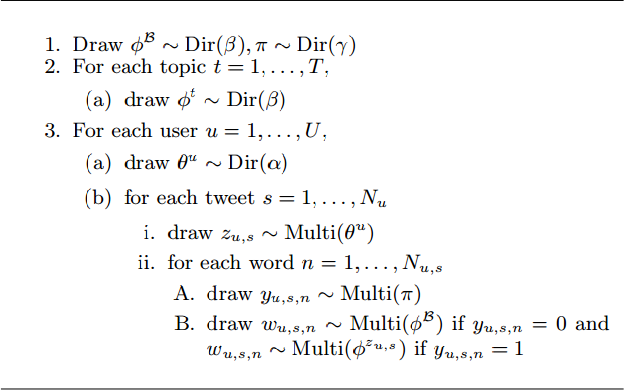
\includegraphics[width=0.6\textwidth]{figures/lda-algo}
 \caption{Twitter LDA Generative Process}
 \label{fig:twitterlda-algo}
\end{figure*}

Formally, let $\theta_u$ denotes the topic distribution for a user $u$. Let $\phi_t$ be the distribution of words for the topic $t$ and let $\phi_B$ be the distribution of background words. $\pi$ is a bernouli distribution which denote the choice of a word to be a background or a topic word. $\alpha~\beta~\gamma$ are dirichlet parameter used for generating respective dirichlet distributions. The plate notation for the model is given in figure \ref{fig:plate} The generative algorithm is given in figure \ref{fig:twitterlda-algo}.
\section{\uppercase{Experiments}}
Parallel to our literature survey on topic detection techniques for Twitter, we have also conducted preliminary experiments on a Twitter dataset having 1.6 million tweets. We preprocessed this data.... Next, we ran LDA on this dataset, with each tweet as a document, without any tweet pooling or aggregation. The topic clusters returned by LDA were noisy, with hashtags, usernames, slangs and keywords from all domains (stop words, mood-related, entities, event related etc.) cluttered together. Another reason for these impure clusters was the fact that users use different and often incorrect, spellings for the same words, resulting in potential assignment of same terms to different topics.

Our preliminary experiments have helped us gain better insight into the topic modeling paradigm, and the issues pertinent to its naive use over Twitter dataset. We are in the process of perfoming preprocessing on Twitter dataset to reduce noise, and experimenting with different variations of LDA to come up with a suitable model which generates meaningful and pure topic clusters.

\section{\uppercase{Phase 2}}
In Phase 2, we plan to conduct more concrete experiments with different variations to topic models to come up with a model that fits our domain well. Parallely, we aim to focus on modeling the evolution of detected events. To this end, we plan to work on techniques to generate event evolution graphs, and employ time-series models to predict future events. 

Event prediction using social media has become very popular in recent years considering the diversity of available data. \cite{asur2010predicting} used Twitter to predict box-office revenues for movies. They used a model based on the number of tweets to predict popularity of a movie; for this they analysed the tweet traffic starting from pre-release period to few weeks post release. Futher, they used sentiment analysis based on text classifiers to separate positive opinions from negative ones on a movie to better predict the box-office revenue. It is observed that positive opinions encourage other people to watch the movie thus having positive effect on revenue. Their research also shows that event predictors based on tweets are better than other predictors. Parralelly, research has been done to predict stock market changes using sentiment analysis of tweets. \cite{bollen2011twitter} has used two mood tracking tools, OpinionFinder which distinguishes positive mood from negative mood using tweet feeds and Google-Profile of Mood States (GPOMS) which classifies moods using tweets on 6 different dimensions. The mood timelines thus obtained are used to predict changes in Dow Jones Industrial Average (DJIA) values.

However, research till now has inherently been constraint to prediction popular events based on sentiment analysis of tweets. There has not been much work which specifically focusses on evolution and prediction of events related to unpopular topics. We wish to understand how standard prediction techniques are insufficient for this task, and come up with suitable modifications to increase their accuracy. One promising approach is to couple the analysis of time-series behaviour of different topics based on the Twitter traffic, with the temporal changes in their correlation with events in other topics. This could potentially result in a model that can accurately predict future pattenrs of the same event, as well as predict the triggering or branching out of other events as its consequence.

\bibliographystyle{apalike}
{\small \bibliography{paper}}

\end{document}

